\documentclass[acmtocl]{acmtrans2m}
%&t&{\tt #}&
%&v&\verb|#|&

% fancybox prevents the TOC from printing
%\usepackage{fancyhdr, fancybox, tabularx, verbatim, epsfig}
\usepackage{fancyhdr, tabularx, verbatim, epsfig}
\usepackage{amssymb,psboxit}
\usepackage{rotating}
\usepackage{tabularx}

\newcommand{\amesos}{{\sc Amesos}}

\acmVolume{0}
\acmNumber{0}
\acmYear{00}
\acmMonth{00}

\newtheorem{interface}{Interface}[section]
\newtheorem{remark}{Remark}

\newcommand{\BibTeX}{{\rm B\kern-.05em{\sc i\kern-.025em b}\kern-.08em
    T\kern-.1667em\lower.7ex\hbox{E}\kern-.125emX}}

\markboth{M. Sala and K. Stanley}{Interfaces to Sparse Direct Solvers}

\title{On the Design of Interfaces to Sparse Direct Solvers}

\author{Marzio Sala and Ken Stanley}

\begin{abstract}
We discuss the design of general, flexible, consistent, reusable and efficient
interfaces to direct solution software libraries for 
systems of linear equations on both serial and distributed memory
architectures. We introduce a set of abstract classes to access
the linear system matrix elements and their distribution, to access vector
elements, and control the solution of the linear system.

We describe a concrete implementation of the proposed interfaces, and we
report numerical results that show that the overhead induced by the
object-oriented design is negligible under typical conditions of usage. We
include examples of applications, and we
comment on the advantages and limitations of the design.
\end{abstract}

\category{D.1.3}{Programming Techniques}{Parallel Programming}
\category{D.2.2}{Software Engineering}{Design Tools and Techniques--{\sl
 Object-oriented design methods}}
\category{D.2.13}{Software Engineering}{Reusable Software--{\sl Reusable
  libraries}}
\category{G.1.3}{Numerical Analysis}{Numerical Linear Algebra--{\sl 
  Sparse, structured, and very large systems (direct and iterative methods)}}
%\terms{Documentation, Languages}

\keywords{Direct Solver Libraries, Object-Oriented Design, Distributed Linear Algebra.}
\begin{document}


\setcounter{page}{1}

\begin{bottomstuff}
Author's address:   \\
Marzio Sala: Department of Computer Science, ETH Z\"urich, CH-8092 Z\"urich,
  Switzerland. \\
Ken Stanley: Department of Computer Science, Oberlin College, Oberlin, Ohio, USA.
\end{bottomstuff}

\maketitle

% --------------------------------------------------------------------------- %
\section{Motivations}
\label{sec:introduction}
% --------------------------------------------------------------------------- %

This paper describes the design and the implementation of 
interfaces to serial and parallel direct solution libraries for
sparse linear systems of type
\begin{equation}
  \label{eq:linear_system}
  A x = b,
\end{equation}
where $A \in \mathbb{R}^{n \times n}$ is a real, square matrix, 
  and $x, b \in \mathbb{R}^{n}$ are the solution and
the right-hand side vectors, respectively. 

Generally speaking,
a direct solution algorithm for (\ref{eq:linear_system}) is any 
technique that computes three matrices, $L$, $D$ and $U$, such that
$P\, A\, Q = L \, D \, U$, where $P$ and $Q$ are permutation matrices
and the linear systems with matrices $L$, $D$ and $U$ are
easy to solve~\cite{golub96matrix}. 
The process of computing these three matrices is called {\sl
  factorization}. Generally, $L$ is a lower triangular matrix, $U$ is an
upper triangular matrix, and $D$ is a diagonal matrix 
(or possibly the identity matrix), and the algorithm adopted for their
computation is some variant of Gaussian elimination method.

The development and implementation of
direct solvers for (\ref{eq:linear_system}) is a
challenging task that has been a subject of research over the
last four decades. 
A brief overview of direct solution algorithms  is given in 
Section~\ref{sec:overview}; however,
the focus of this article is on the {\sl usage} of direct solution methods,
    rather than on their development or analysis.
Therefore, the point of view is the one
of application developers (users), interested in solving
(\ref{eq:linear_system}) using already available software libraries.  

\smallskip

Direct solution methods are required by several numerical algorithms, even
within the same application. An
incomplete list would include implicit time-stepping schemes, 
Newton-like methods, multilevel and domain decomposition preconditioners. 
In contrast with serial dense solvers, where one can take advantage of the
widely-available suite of solvers contained in the LAPACK
library~\cite{lapack-guide}, and to distributed dense solvers, where one can
adopt the ScaLAPACK library~\cite{scalapack-guide} or the PLAPACK
library~\cite{alpatov97plapack}, there is no single direct solve library of
choice for (distributed) sparse linear systems.  Since no ``gold
standard'' exists, application developers aiming to solve
(\ref{eq:linear_system}) have to look
for the library best optimal to their purposes. This search is affected by the following questions:
\begin{enumerate}
\item[(Q1)] is the software library easy to use?
\item[(Q2)] is it well documented?
\item[(Q3)] is it actively supported, does its interface change over time?
\item[(Q4)] is it reliable and robust?
\item[(Q5)] is it efficient in terms of CPU time?
\item[(Q6)] how much storage does it require?
\end{enumerate}
The relative importance of these aspects is somehow subjective. For relatively
simple problems, (Q5) is usually the key point, followed by (Q6). For
complicated problems, and especially in industrial applications, (Q4) is of
paramount importance. Points (Q1), (Q2) and (Q3) are usually considered as
``technical details'' of minor importance, even if they aren't. 
In fact, library developers often include a wide variety
of choices, aiming to provide a powerful and comprehensive library.
Application developers, instead, are usually not experts in the domain, and do
not aim to become such. They often choose the code that looks easier to use and
seems to perform in a reasonable way. This difference of views creates a gap between
the actual and potential use of mathematical software.
Of course, a simple but inefficient library is of no use; therefore the
``optimal'' library will exhibit a mixture of the features outlined above.

Once a library has been chosen, the application developers have to
write a custom-made interface between the selected library and
the application. This usually requires storing the linear system matrix $A$
using the
  storage format required by the library, then calling the correct sequence of
  instructions to factorize the matrix and solve the linear system.  In our
  opinion, the approach is sub-optimal for both application and library
  developers because it:
\begin{itemize}

\item 
{\sl offers partial coverage}. Writing a custom-made interface means that only the
targeted library will be used.
This is inconvenient because of the already mentioned difficulty to choose
{\sl a-priori} the best library for a given application.
In some cases, a theoretical analysis of
the problem at hand can suggest the right algorithm. Alternatively, one can
consider numerical comparisons on test matrices available in the literature,
see for instance \cite{amestoy01analysis,gupta01recent} and
the references therein. Often, however, one has to validate
a given library on the application, architecture, and data
set of interest, and this can be done only if the interface  to a library
is already available;

\item 
{\sl produces maintenance problems.}
Including the interfaces within the application code requires the application
developers to manipulate the matrix format, the memory
management, the calling conventions, and others, that can vary 
from one library to the following. Although not necessary difficult, these
activities are usually time-consuming;

\item 
{\sl delays the usage of new libraries.} 
Large application codes usually have a long life.  The sheer size of
the codes and a natural reluctance to change a successful code discourage any
effort of rewriting unless absolutely necessary.
Since a new library 
(or a new version of a given library) may require a new matrix format or
distribution, or a new calling convention, users may simply decide to continue
using the interface already developed.
\end{itemize}

This article shows that it is possible to overcome all these problems by using
modern software techniques and resorting to object-oriented (OO) design and
programming.  We propose a set of clean, consistent and easy-to-use interfaces
between the application and the direct solver libraries.  Each interface takes
care of dealing with the direct solver library, in a manner that is
transparent to the application developers, and automatically manages matrix
formats, data layout, calling conventions, and everything else is
required by the supported libraries. 

The basic ideas of our design are indeed quite old, and can be traced back to
almost 30 years ago~\cite{duff79performance,george79design}. More recently,
  articles~\cite{george99object,dobrian99design} discussed the usage of
  abstract interfaces and OOD for the direct solution of sparse linear
  systems.  We extend these ideas by abstracting the concepts to
a higher level, and making the interfaces independent of the supported
libraries. The interfaces are presented and implemented as a
set of C++ classes.  C++~\cite{cppbook}
supports object-oriented programming, and it is relatively easy to interface
FORTRAN77, FORTRAN90 and C libraries with C++ code. The C++ language
supports abstraction through classes, inheritance and polymorphism. For
application developers, abstraction is important because brings simplicity,
by allowing components with a minimalistic interface. It also ensures flexibility
because it decouples the different algorithmic phases from the data structures.
Finally, abstraction allows extensibility in the sense that new (yet to
                                                                develop)
libraries can be easily added, at almost no cost to the application developer.
Another candidate language could have been FORTRAN90, but it does not have
inheritance and polymorphism.

%
%  I think that we can be more direct about our dependence on MPI here.  
%
As of the parallel computing mode, 
we consider parallel architectures with distributed memory, and we suppose
that the message passing interface MPI~\cite{gropp98mpi} is adopted.
This approach is followed by some scientific libraries, see
\cite{heroux05trilinos,petsc-user-ref,falgout02hypre}. As a result, the presented
design can be easily interfaced with the aforementioned projects.

\smallskip

The paper is organized as follows. Section~\ref{sec:overview} introduces the
basic concepts of direct solution algorithms. Section~\ref{sec:design}
describes the requirements and the design of the proposed
interfaces. A concrete implementation is addressed in
Section~\ref{sec:concrete}. Section~\ref{sec:numerical} reports some
numerical results that quantify the overhead required by the generality of
the approach. Two
examples of application are reported in Section~\ref{sec:example}.
Section~\ref{sec:conclusions} outlines the conclusions.

%-----------------------------------------------------------------------------
\section{Brief Overview of Direct Solution Methods}
\label{sec:overview}
%-----------------------------------------------------------------------------

This section gives a broad view of the problematics of Gaussian elimination
algorithms for distributed sparse linear systems. 
Following~\cite[Chapter 6]{dongarra98numerical}, a direct solution algorithm
for sparse matrices can be divided in the following phases:
\begin{itemize}
\item[(S0)] a preordering phase that exploits structure;
\item[(S1)] an analysis phase where the matrix structure is analyzed to produce a
suitable ordering and data structures for efficient factorization;
\item[(S2)] a factorization phase where the numerical factorization is performed;
\item[(S3)] a solve phase where the factors are used to solve the system using
forward and backward substitution.
\end{itemize}
Some codes combine phases (S1) and (S2). Phase (S2) usually requires the most
computing time, while phase (S3) is generally one order of magnitude faster.
Phase (S0) is typical of sparse matrices:
since $A$ is sparse, $L$ and $U$ are typically sparse, though they may have some
fill-in, i.e. non-zero entries which are zero in $PAQ$.  
In a typical solver for an unsymmetric matrix, the column permutation,
$Q$ is chosen to minimize fill-in, while $P$, the row permutation, is
chosen to maintain numerical stability.  
%Pivoting for numerical
%stability makes it impossible to know in advance how the algorithm
%will proceed and requires a flexible data structure.  This is
%particularly difficult for distributed memory codes.  
Many ordering methods exist to reduce fill-in, for example multiple variations
on minimum degree orderings and graph partitioning algorithms.  Solvers
designed for symmetric and nearly symmetric matrices typically use symmetric
permutations to maintain symmetry.  No single ordering method is best for all
matrices, nor has a heuristic been found that consistently chooses the best
ordering~\cite{BaumannFleischmannMutzbauer03,AmestoyDavisDuff03}. 

Since pivoting adds complexity which significantly increases execution
time, many solvers offer options to reduce the cost of pivoting~\cite{LiDemmel509092,sg:04-fgcs}.  Some
equilibrate the rows and columns of the matrix to improve diagonal
dominance.  Many codes will consider the effect on execution time when
choosing a pivot, accepting some loss of numerical stability~\cite{Malard126136}.
Typically this just means accepting the diagonal pivot if it is within
some threshold of the best available, but some codes will take the
predicted effect on execution time into consideration when choosing an off
diagonal pivot~\cite{Davis992205}.

It is possible to combine similar rows and columns into blocks to improve
locality and allow high performing BLAS to be called; this combination can
consider only rows and columns that are identical, or accept minor differences
in the rows and columns that they treat as blocks.  Such blocking can reduce
the cost of symbolic factorization as well~\cite{amestoy01analysis}.

The performance of a sparse direct solver depends on the underlying
matrix, computer, application, algorithms, and libraries as well as
the code and how it is compiled.  
Given the differences in matrix, computer, application, algorithms,
and libraries, it is unlikely that a single sparse direct solver will 
outperform all others across all usages.  

For more details on the subject, the interested reader should
consult the specialized literature, for
example~\cite{duff86direct,duff97sparse} and the references therein. 


%Although a solver designed for an
%unsymmetric matrix will work on symmetric matrices, solvers designed
%for symmetric matrices will typically be faster on symmetric matrices.
%Codes designed for shared memory computers will not run on distributed
%memory computers.  Codes designed for distributed memory computers can
%work on shared memory computers, but cannot take full advantage of the
%shared memory architecture.  Many applications require repeated solves
%with little or no difference in the matrix between solves.  Some
%algorithms are able to take advantage of the similarity in matrices
%between solves.

%The different characteristics of the matrices which users wish to
%solve impact sparse direct solvers.  Some matrices are symmetric in both
%structure and data $A_{i,j} = A_{j,i}$ for all $i$ and $j$.  Some of
%the symmetric matrices are positive definite, SPD, and require no
%pivoting.  The most efficient algorithms for symmetric and SPD
%matrices will not work on other matrices.  Some matrices are symmetric in
%structure, $A_{i,j} == 0$ iff $A_{j,i} == 0$, or nearly so.
%Algorithms that maintain symmetry typically outperform others on
%matrices with symmetric or nearly symmetric structure.  Some matrices have many
%columns and/or rows that are structurally identical, or nearly so.
%Aggregating nearly identical rows and columns into blocks allows more
%efficient BLAS3 routines to be used.  Some matrices can be factored with little
%fill-in, others require significant fill-in.  Matrices that can be
%factored with little fill-in and have few identical or nearly identical
%rows and columns are best handled by a low overhead code that does not
%use the BLAS.  Some matrices are banded or nearly so, allowing the use
%of a banded solver.  Matrices that have a non-trivial reduction to
%block triangular form can be solved more quickly, often dramatically,
%by a solver that includes reduction to block triangular form.  No sparse direct solver is best for all types of matrices.  
%
%% MS % This seems to generic to me... Maybe re-write?  
%Some sparse direct solvers are designed for single processor
%computers, some are designed for shared memory computers and others
%are designed for distributed memory computers.  Solvers designed for
%single processor computers can, if they use the BLAS for much of their
%computation, achieve some speedup on shared memory computers.
%Likewise, solvers designed for distributed memory computers can work
%on shared memory computers using an MPI interface.  However, only
%codes designed for shared memory computers can take advantage of the
%shared memory architecture.  Codes designed for shared memory
%computers will not work on distributed memory computers.  No single
%code will provide optimal performance across all architectures.

%Some solvers handle certain application requirements better than
%others.  Most applications perform a series of solves, possibly
%involving similar or even identical matrices.  If the matrix does not
%change between two consequetive solves, the symbolic and numeric
%factorization phases need not be performed for each solve.  If the
%structure of the matrix does not change between consequetive solves,
%but the values do, the numeric factorization must be performed for
%each solve, though the symbolic factorization phase need not be.  If
%the matrix values change, but the change is modest, the pivot order
%may not need to change.  Therefore, some applications care most about
%the execution time of the solve phase, while others are most sensitive
%to the execution time of the factorization (numeric and/or symbolic).
%Some applications require more accuracy than others.

%The three common methods for exploiting parallelism are the
%multi-frontal method, coalescing  similar 
%columns into blocks and calling a parallel dense solver 
%to factor the final block of the matrix~\cite{amestoy01analysis}.

% MS % discussed in the conclusions: skip it here?
%
% Some solvers allow incomplete factorizations which ignore small
% elements in the original matrix and/or the $L$ and $U$ factors.
% This feature is used primarily by users seeking a
% preconditioner for an iterative method.

%Some solvers use iterative refinement to improve accuracy.  Iterative
%refinement is used most often with codes that do not perform full partial pivoting.  

%-----------------------------------------------------------------------------
\section{Project Design}
\label{sec:design}
%-----------------------------------------------------------------------------

%\begin{table}
%\begin{center}
%\begin{tabular}{| l | c c c l l | p{4cm} |}
%\hline
%package & 
%\rotatebox{90}{complex} &
%\rotatebox{90}{parallel} &
%\rotatebox{90}{out-of-core} &
%\rotatebox{90}{language} &
%method &
%references \\
%\hline
%%
%CHOLMOD     & $\bullet$ & -- & -- & C & left-looking supernodal &
%\cite{davis05cholmod} \\
%%
%DCSPACK     & $\bullet$ & -- & D & C & multifrontal & \cite{dscpack-manual} \\
%%
%KLU         & $\bullet$ & -- & -- & C & left-looking & \cite{davis05klu} \\
%%
%Mathematica & $\bullet$ & -- & -- & -- & various & \cite{wolfram99mathematica} \\
%%
%MATLAB      & $\bullet$ & -- & -- & -- & various & \cite{gilbert92sparse} \\
%%
%MUMPS       & $\bullet$ & D & -- & F90 & multifrontal & \cite{mumps-manual} \\
%%
%Oblio       & $\bullet$ & -- & $\bullet$ & C++ & left, right, multifrontal &
%\cite{dobrian00oblio} \\
%%  
%PARDISO     & $\bullet$ & S & -- & C & left/right supernodal  & \cite{oskl:04-etna,sg:04-fgcs} \\
%%
%%%PaStiX      & $\bullet$ & D &  ?? & -- & left-looking supernodal & \cite{henon00pastix} \\
%%
%TAUCS       & $\bullet$ & S & $\bullet$ & C & left-looking, multifrontal &
%\cite{irony04parallel,rotkin04design,rozin04locality} \\
%%
%UMFPACK     & $\bullet$ & -- & -- & C & multifrontal & \cite{umfpack-home-page} \\
%%
%SPOOLES     & $\bullet$ & S/D & -- & C & left-looking, multifrontal & \cite{ashcraft99spooles} \\
%%  
%SuperLU     & $\bullet$ & -- & -- & C & left-looking supernodal &  \cite{superlu-manual} \\
%%
%SuperLU\_DIST & $\bullet$ & S & -- & C & left-looking supernodal &  \cite{superlu-manual} \\
%SuperLU\_DIST & $\bullet$ & D & -- & C & right-looking supernodal & \cite{superlu-manual} \\
%WSMP & $\bullet$ & S/D & -- & binaries & multifrontal & \cite{gupta02improved} \\
%%%Y12M & -- & -- & -- & F77 & right-looking Markowitz & \cite{y12m} \\
%
%
%\hline
%\end{tabular}
%\caption{Package features. `--' means that the feature is not supported. `S'
%  indicates support for shared memory machines, `D' for distributed memory
%    machines.}
%\label{tab:packages}
%\end{center}
%\end{table}

An analysis of currently available direct solver libraries can be found
in \cite{davis05summary}; see also~\cite[Section 6.7]{dongarra98numerical}.
A closer look at these solvers reveals the following major
differences:
\begin{itemize}
\item {\sl different programming languages are used,} even if most projects are
written in C;

\item {\sl different communication paradigms are used.} 
 Most of the reviewed libraries are serial, some are based on the MPI
 paradigm, others take advantage of shared memory computers;

\item {\sl different matrix formats and data layout are used;}

\item {\sl different algorithms are used.} The underlying algorithms do
considerably differ
and can therefore perform differently, depending on the considered matrices and
computer architectures.

\end{itemize}

Despite these differences, all solvers are accessed with a sequence of
steps similar to steps (S0)--(S1) of Section~\ref{sec:overview}:
\begin{enumerate}
\item[(A1)] Definition of the sparsity pattern of the linear system matrix;
\item[(S0/S1)] Computation of the symbolic factorization, which includes
preordering and analysis. The
symbolic factorization refers to all operations that can be performed by
accessing the matrix structure only (without touching the values of the matrix entries);
\item[(A2)] Definition of the values of the linear system matrix;
\item[(S2)] Computation of the numeric factorization, that is, the computation
of the entries of the factored terms;
\item[(A3)] Definition of the right-hand side;
\item[(S3)] Solution of the linear system for given $x$ and $b$.
\end{enumerate}
Steps (A1), (A2) and (A3) are application-dependent; 
our aim is to standardize steps (S0/1), (S2)
and (S3) to allow a transparent and consistent usage of all libraries. This
can be done by adding an intermediate layer between the application and the
libraries. This layer will be defined in terms of an abstract framework, that
satisfies the following requirements:
\begin{itemize}

\item {\sl simplicity of usage:} Solving linear system (\ref{eq:linear_system}) in a language
like MATLAB is very easy, i.e.~one just writes \verb!x = A \ b!. It should not be much
more difficult in a production code;

\item {\sl flexibility:} More than one algorithm/library must be available,
  for both serial and parallel architectures;

\item {\sl efficiency:} The overhead due to the framework must be minimal.
\end{itemize}

To satisfy these goals, we introduce a set of abstract classes, which will be
used to define interfaces to the data layout of distributed objects, 
vectors, matrices, linear system, and the solver.
These classes are reported as C++ classes, but the concepts are more general
and the discussion is largely language-independent.

\smallskip

The first class that we need to introduce is a {\tt Map}, defined by
\begin{interface}
\label{int:map}
The {\tt Map} class will contain the following methods:

\begin{itemize}
\item {\tt int GetNumMyElements()} returns the number of locally owned elements;
\item {\tt int GetNumGlobalElements()} returns the global number of elements;
\item {\tt int GetGID(const int LID)} returns the global ID of the local node {\tt ID}.
\end{itemize}
\end{interface}
A {\tt Map} defines the local-to-global numbering. We require that any global
ID is assigned to exactly one processor. {\tt Map}'s are used to define the
layout of distributed vectors and matrices. The next class is the {\tt Vector}
class, which specifies the interfaces for
distributed vectors\footnote{
For the sake of simplicity, this paper focuses on vectors and not on
multi-vectors, that is, a collection of vectors with the same {\tt Map}.
However, the presented design can be straightforwardly extended to tackle
multi-vectors as well.
}. We assume that {\tt Vector}'s  locally exist as a {\tt double} arrays.
A simple set of methods for the {\tt Vector} class is reported by 
\begin{interface}
\label{int:vector}
The {\tt Vector} class will contain the following methods:

\begin{itemize}
\item {\tt double* GetValues()} returns a pointer to the local array of values;
\item {\tt const Map\& GetMap()} returns a reference to the underlying Map object.
\end{itemize}
\end{interface}

As regards the linear system matrix $A$, we do not impose a matrix format,
rather we specify an abstract interface to {\sl query} for matrix elements. 
The only assumption is
that the storage format adopted by the application allows a fast access to all
the nonzero elements in a given (locally owned) row.
This class, called {\tt RowMatrix}, is a fairly general sparse matrix 
interface. For
distributed matrices, we assume that each row is owned by exactly
one processor; rows can be distributed in arbitrary ways among the available
processors. As such, the locally owned matrix can be decomposed as
\begin{equation}
A^{(loc)}_i + A^{(ext)}_i,
\end{equation}
where $A^{(loc)}_i$ represents the square submatrix of elements whose row
and column correspond to locally hosted rows, while
$A^{(ext)}_i$ contains matrix elements with locally owned rows and
non-locally owned columns. The
columns contained in $A_i^{(ext)}$ are usually called {\sl ghost nodes}.
The abstract matrix interface is as
follows.
\begin{interface}
\label{int:ami}
The abstract interface to the distributed square matrix $A$
will contain the following methods:
\begin{itemize}
\item \verb!int GetNumMyRows()! returns the number of locally hosted rows;
\item \verb!int GetNumGlobalRows()! returns the global number of rows;
\item \verb!int GetNumGhostNodes()! returns the number of ghost nodes;
\item \verb!void UpdateMyGhostNodes(Vector& x)! updates the values of ghost nodes
 in the input vector {\tt x};
\item {\tt int GetNumMyRowEntries(const int ID)} returns the number of nonzero of
the (locally owned) row {\tt ID};
\item {\tt void GetMyRow(const int ID, const int Length, int\& NumEntries, int* Indices, double*
                             Values)} copies the
column IDs and values of all nonzero elements of the locally hosted row {\tt
  ID} in the user's allocated arrays (of length {\tt Length}). The output
  variable {\tt NumEntries} returns the number of nonzeros in the row;
\item \verb!const Map& GetRowMap()! returns a reference to the map;
\item \verb!bool IsSymmetric()! returns {\tt true} is only the upper
triangular part of the matrix is accessed through {\tt GetMyRow()}, {\tt
  false} otherwise.
\end{itemize}
\end{interface}
Interface~\ref{int:ami} defines a standard set of methods to ``view'' matrix
elements through row extractions. This approach is used, 
for instance,
in~\cite{Epetra-Ref-Guide,ml-guide,duff02overview,lujan00oolala}. We decided
not to adopt iterators in {\tt GetMyRow()} to make the code easier to use.
Besides, since this method will be mostly used to convert the matrix into a
specific solver's format, the use of iterators would have not increased the
performances.

\smallskip

We now specify the basic requirements for the interface to a linear problem.
\begin{interface}
\label{int:lp}
The {\tt LinearProblem} interface
will contain the following methods:
\begin{itemize}
\item \verb!void SetMatrix(RowMatrix* A)! sets the linear system matrix;
\item \verb!void SetX(Vector* x)! sets the solution vector;
\item \verb!void SetB(Vector* b)! sets the right-hand side vector;
\end{itemize}
\end{interface}
Interface~\ref{int:lp} can be easily extended to 
standarize operations like scaling or reordering.

%\smallskip

%The last utility class we need to introduce is the {\tt Redistribute} class.
%We suppose that, given two maps, called {\tt SourceMap} and {\tt TargetMap}, a
%{\tt Redistribute} object can be used to redistribute a {\tt Vector} based on
%{\tt SourceMap} to a vector based on {\tt TargetMap}. This class encapsulates
%all the complexity of data communication.

\smallskip

Finally, we can introduce the {\tt solver} interface class, which is defined as
follows:
\begin{interface}
\label{int:asi}
The {\tt Solver} interface
will contain the following methods:
\begin{itemize}
\item \verb!void SetLinearProblem(LinearProblem* LP)! sets the linear problem
to solve;
\item \verb!void SetParameters(List)! specifies all the parameters for the solver;
\item \verb!int SymbolicFactorization()! performs the symbolic factorization, that
is, all the operations that do only require the matrix graph and not the
actual matrix values;
\item \verb!int NumericFactorization()! performs the numeric factorization, that
is, it computes the matrices $L$, $D$ and $U$ by accessing the matrix values.
Both the solution and the right-hand side vectors are not required in this phase;
\item \verb!int Solve()! solves the linear system. This phase requires the
solution and the right-hand side vectors.
\item \verb!void GetParameters(List)! returns a list of output parameters, to
provide feedback from the supported library.
\end{itemize}
\end{interface}

A flowchart of the factorization processes within a typical application
is reported in Figure~\ref{fig:flowchart}.
\begin{figure}
\begin{center}
\fbox{ 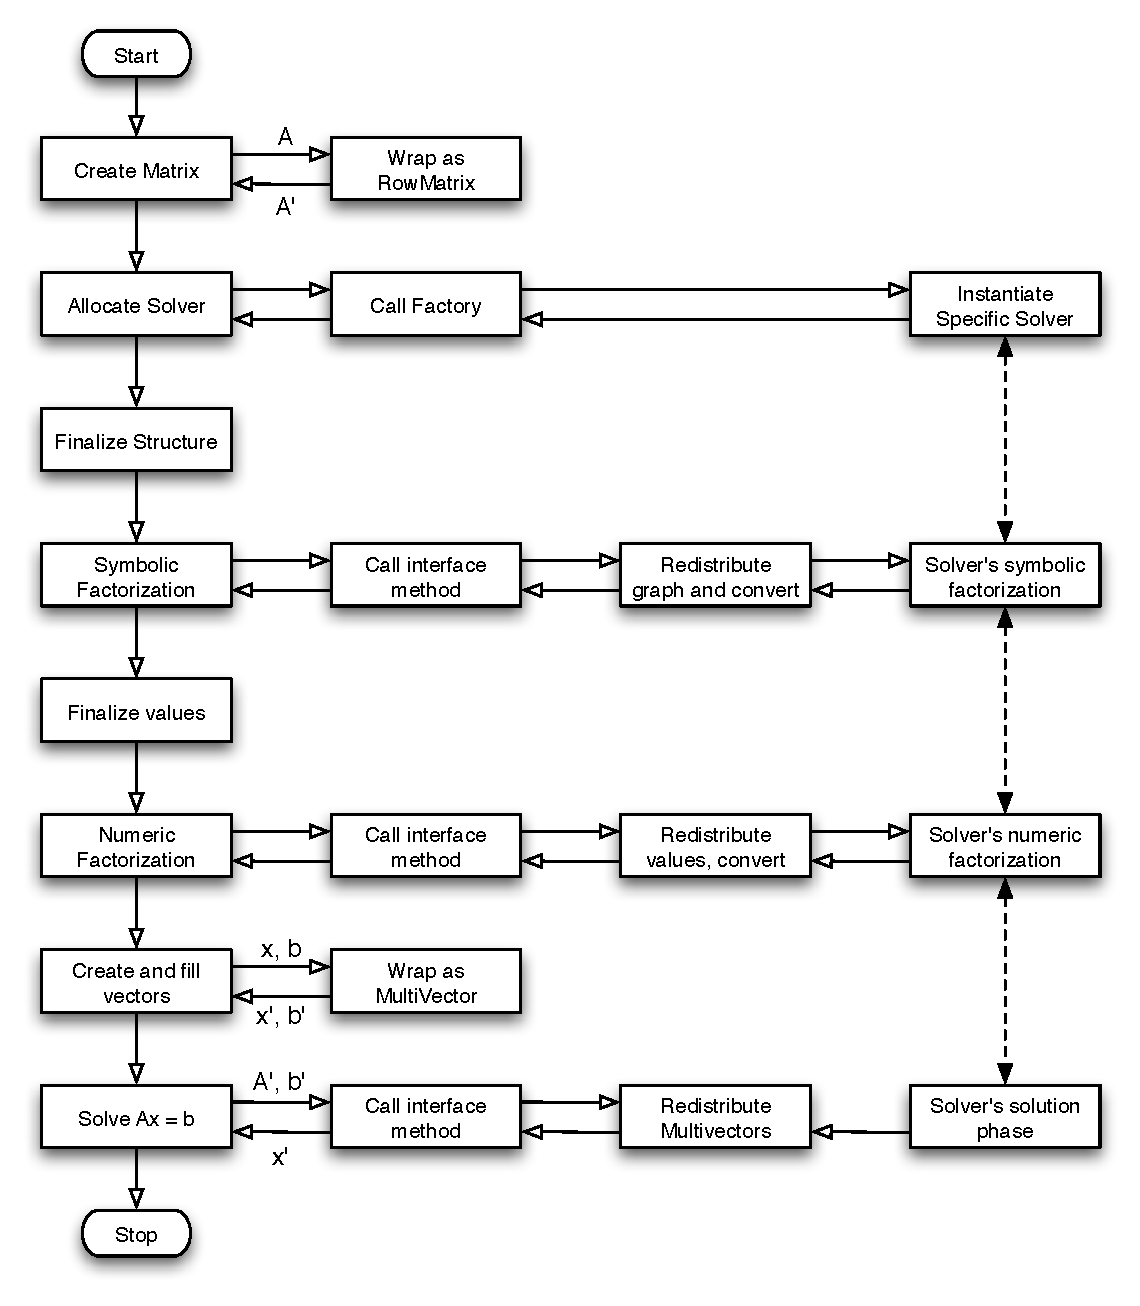
\includegraphics[width=12cm]{amesos_flowchart.pdf}}
\end{center}
\caption{Flowchart of linear system solution. $A, x$ and $b$ represent objects
  defined in the application, while $A', x'$ and $b'$ are the corresponding 
    wrappers that
    satisfy Interfaces~\ref{int:vector} and \ref{int:ami}. Dashed lines mean
    that a given phase uses data defined in another phase. From left to right,
  the first column 
    represents phases occurring in the application; the second column wrapping
and calls to generic interface methods; the third column actions
occurring in the solver interface, while the fourth column calls to supported
direct solver library.}
\label{fig:flowchart}
\end{figure}

%------------------------------------------------------------------------- 
\section{A Concrete Implementation}
\label{sec:concrete}
%------------------------------------------------------------------------- 

We now describe a concrete implementation of the interfaces of
Section~\ref{sec:design}, as implemented in
the {\sl \amesos}\footnote{
\amesos\ is a Greek term that loosely translated means ``direct.''} package~\cite{Amesos-Reference-Guide}.
\amesos,
developed by (in alphabetical order) T.~Davis, M.~Heroux, R.~Hoekstra, 
M.~Sala, and K.~Stanley. \amesos\ is distributed within the
Trilinos project~\cite{heroux05trilinos}.
To increase portability, \amesos\ is configured using autoconf and autotools;
each solver can be enabled or disabled at configure time. Users can take
advantage of the bug-tracking tool Bugzilla to provide feedback or request
improvements.

We have considered the following direct solvers:
  KLU\footnote{The sources of KLU are
  distributed within \amesos.} \cite{davis05klu}, 
  UMFPACK~\cite{umfpack-home-page}, SuperLU and
  SuperLU\_DIST~\cite{superlu-manual}
  DSCPACK~\cite{dscpack-manual}, 
  MUMPS~\cite{mumps-manual}, 
  TAUCS~\cite{irony04parallel,rotkin04design,rozin04locality}, 
  and PARDISO~\cite{oskl:04-etna,sg:04-fgcs}. An interface to MA28 is
  under development.
These libraries use different algorithms that are
representative of a far wider range of codes. Also, these supported libraries are
among the best codes publicly available, and are widely used.  

\amesos\ also includes interfaces to LAPACK and ScaLAPACK. The rationale is
that
sparse libraries are much more complicated than libraries for dense systems,
  and the question of how much is gained with respect to dense solvers 
  is often asked. Dense
  solvers are usually more robust than sparse solvers and could be used as
  last-resort in extreme cases.  By adding support for LAPACK and ScaLAPACK, 
  users can experiment with these
  solvers, which might outperform  sparse libraries in some cases 
  (for instance, if applied to small matrices, or almost dense matrices). 

\begin{figure}
\begin{center}
\begin{tabular}{| p{12cm} | }
\hline
 \\
\begin{minipage}{12cm}
\begin{verbatim}
#include "Amesos.h"
#include "mpi.h"
#include "Epetra_MpiComm.h"
...

int main(int argc, char *argv[]) 
{
  MPI_Init(&argc, &argv);
  Epetra_MpiComm Comm(MPI_COMM_WORLD);

  Epetra_Map* Map = <create map here, Interface 3.1>;
  Epetra_MultiVector* x = <create solution vector here, Interface 3.2>;
  Epetra_MultiVector* b = <create right-hand side here, Interface 3.2>; 
  Epetra_CrsMatrix* A = <create matrix here, Interface 3.3>;

  Epetra_LinearProblem Problem(A, x, b); // Interface 3.4

  Amesos Factory;                  // factory class
  string SolverType = "Umfpack";   // selected interface
  Amesos_BaseSolver* Solver;       // generic solver object, Int. 3.5
  Solver = Factory.Create(SolverType, Problem);

  Teuchos::ParameterList List;     // allocate container for params,
  List.set("PrintTiming", true);   // set one in the container, then
  Solver->SetParameters(List);     // pass the container to the solver

  Solver->SymbolicFactorization(); // symbolic factorization
  Solver->NumericFactorization();  // numeric factorization
  Solver->Solve();                 // linear system solution
  delete Solver;
    
  MPI_Finalize();
  return(EXIT_SUCCESS);
} // end of main()
\end{verbatim}
\end{minipage} \\
 \\
 \hline
\end{tabular}
\caption{Example of code using \amesos. The code uses the \amesos\ interface to
  UMFPACK to solve the linear system. The creation of the matrix, solution and
    right-hand side are not reported.}
\label{fig:example}
\end{center}
\end{figure}

\amesos\ defines Interface~\ref{int:asi}, as well as all its concrete
implementations (for a little more than 13.000 code lines, including comments
                 and Doxygen documentation), and it
takes advantage of the {\sc Epetra} package~\cite{Epetra-Ref-Guide} to specify
Interfaces~\ref{int:map}, \ref{int:vector}, \ref{int:ami} and \ref{int:lp}.
{\sc Epetra} defines several concrete implementations of
Interface~\ref{int:ami}, making it easy to read matrices from formats
  like AIJ or CSR.
The Standard Template Library (STL)~\cite{wise96overview} is used
to increase performances whenever possible.
The \amesos\ implementation of Interface~\ref{int:asi} also contains methods
{\tt PrintStatus()} and {\tt PrintTiming()} that offer a standard way to
access various statistics and timings for all packages.

An example of usage of \amesos\ is reported in Figure~\ref{fig:example}. 
Although this particular example requires MPI, \amesos\
can be compiled with or without support for MPI. (Clearly, distributed
solvers are available only when compiled with MPI support.) The only
\amesos\ include is \verb!Amesos.h!, which does not include the header files of
the supported library. The required interface is specified by the string
variable \verb!SolverType!, and is created by using the
factory class \verb!Amesos!. Factory classes are a programming
tool~\cite{alexandrescu01modern} that implement a sort of ``virtual
constructor,'' in the sense that one can instantiate a derived (concrete) object
while still working with abstract data types. 
The example reported in Figure~\ref{fig:example} adopts UMFPACK as a solver; 
by using the factory class, other
interfaces can be created by simply changing the parameter
{\tt SolverType}. Note that the supported solver can be serial or parallel,
  dense or sparse: the user code still remains the same, except for the name
  of the solver;
  \amesos\ will take care of data redistribution if required by the selected
  solver. 

\begin{figure}
\begin{center}
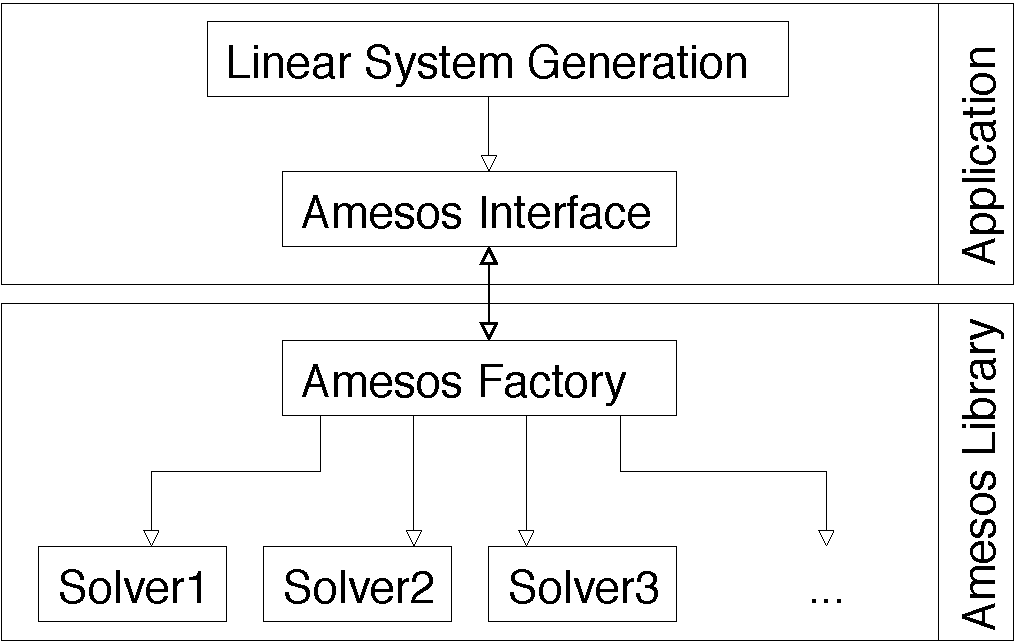
\includegraphics[width=6cm]{amesos_and_application.pdf}
\end{center}
\caption{Connection between a generic application and \amesos.}
\label{fig:app}
\end{figure}

A generic interface between an application code and \amesos\ is as represented
in Figure~\ref{fig:app}: Once $A$, $x$ and $b$ of (\ref{eq:linear_system}) are
available, the application can use the factory class to access the supported
libraries.

Each \amesos\ interface automatically selects the default parameters defined by
the supported solver. In most cases, these values are a robust and reliable
choice for most applications. If required, the user can tune some of the
parameters by using the method \verb!SetParameters()!. The list of supported
parameters is reported in~\cite{Amesos-Reference-Guide}.

% ------------------------------------------------------------------------
\section{Numerical Results}
\label{sec:numerical}
% ------------------------------------------------------------------------

The example code of Figure~\ref{fig:example} has shown the facility of usage
of \amesos; this section, instead, aims to quantify its overhead.

Figure~\ref{fig:results} reports the percentage of CPU time required by the
\amesos\ interface with respect to the time required by the underlying
library. We have considered the SuperLU and UMFPACK interface for the solution
of all matrices in the FIDAP collection, available
at~\cite{boisvert97matrix}. The matrix sizes range from 27 
({\tt FIDAP005}) to 22294 ({\tt FIDAPM11}). All problems are solved using one
1.67 GHz G4 processor with 1024 Mbytes of RAM, running MAC OS X 10.4 and gcc
4.0.0. The table reports the percentage of the CPU time required by the
interface with respect to the time required by the considered solver, and
quantifies the overhead required by \amesos. We have used the default set of
parameters for both solvers.

As expected, for small matrices (for example \verb!FIDAP005! or \verb!FIDAPM05!, of size
27 and 42, respectively) 
the overhead is considerable. When considering bigger matrices ($n > 3000$),
then the overhead is  always below 5\%. All the overhead is spent in
converting the matrix to the abstract format of Interface~\ref{int:ami} to the
format required by the library, and performing additional safety checks.
Note that this overhead can indeed be reduced by adding specialized classes,
     that satisfies Interface~\ref{int:ami} but internally stores the matrix
     in the format required by a given solver library. Solvers derived from
     Interface~\ref{int:asi} can perform a {\tt dynamic\_cast}, and then get
     the already allocated data structure containing the matrix. This solution
     is inelegant and it requires knowledge of derived classes in the solver
     interface, but can greatly increase performance.  Vectors are less
     problematic since Interface \ref{int:vector} already offers the ability
     to get the raw pointers required by the supported library. However, these
     vectors may need to be redistributed to match a given solver's
     requirements.

\begin{figure}
\begin{center}
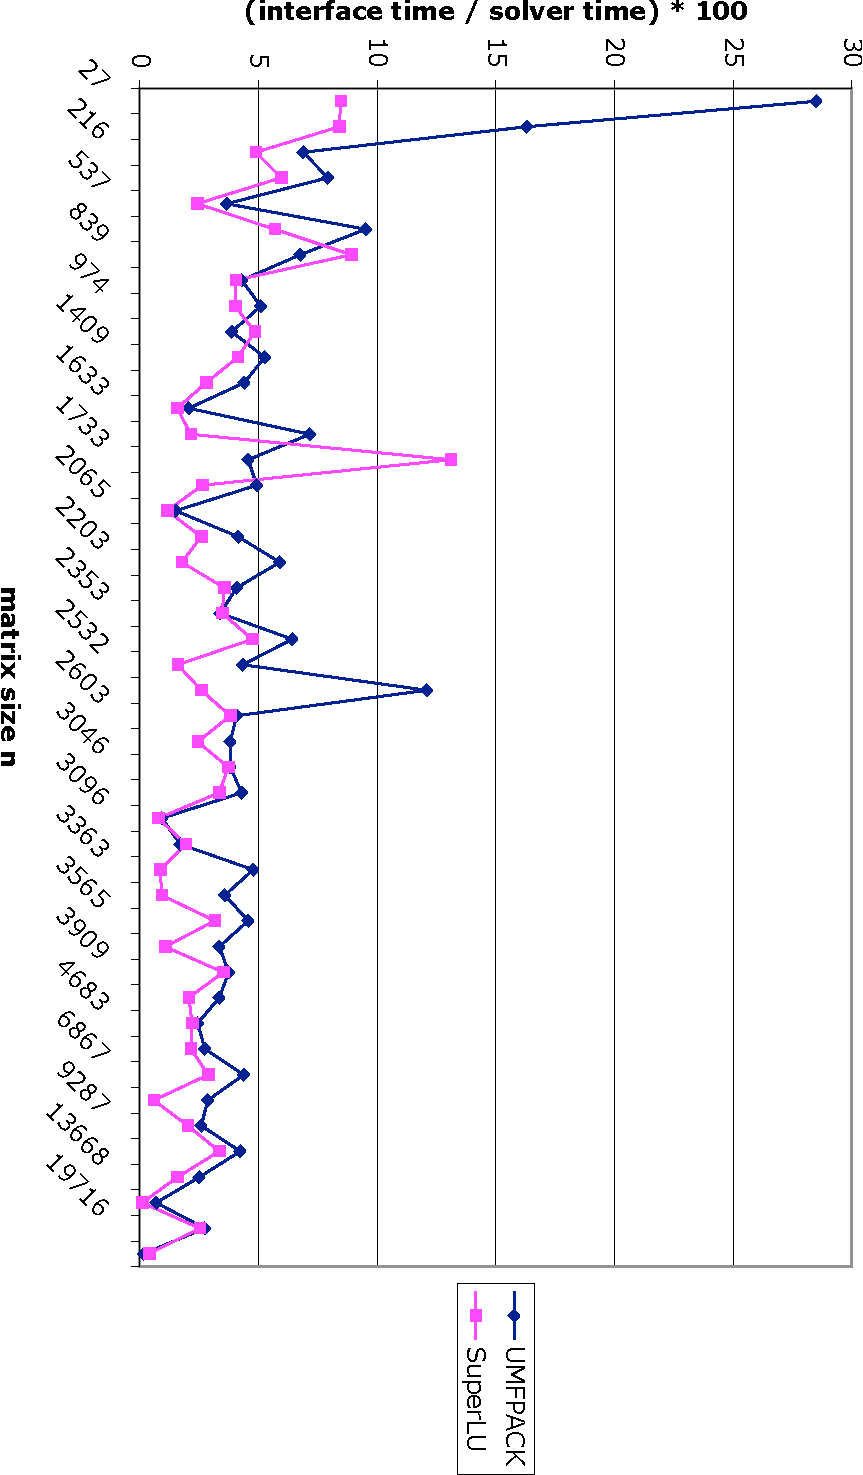
\includegraphics[angle=90,width=12cm]{interface_time.pdf}
\caption{Additional time required by the \amesos\ interface with respect to the
time required by the solver, for different matrices and solvers. $n$
  represents the size of the matrix, and $nnz$ the total number of nonzeros.
The results were obtained on a G4 1.67 GHz with 1 GByte of RAM.}
\label{fig:results}
\end{center}
\end{figure}

%-----------------------------------------------------------------------------
\section{Examples of Applications}
\label{sec:example}
%-----------------------------------------------------------------------------

%-----------------------------------------------------------------------------
\subsection{Applications to Domain Decomposition and Multilevel Preconditioners}
\label{sec:preconditioner}
%-----------------------------------------------------------------------------

From an abstract point of view, an algebraic domain decomposition
preconditioner for the iterative solution of the linear system
(\ref{eq:linear_system})
is any preconditioner $B$ that can be written as
\begin{equation}
\label{eq:prec}
B^{-1} = \sum_{i=1}^M P'_i {A'_i}^{-1} R_i,
\end{equation}
where
$M$ is the number of subdomains, $R_i$ is the restriction to subdomain $i$,
  $P_i = R_i^T$, $P_i'$ an auxiliary prolongator operator, and 
$A'_i$ an approximation to $A_i = R_i A P_i$.  We refer to 
monographs~\cite{QV2,smith96parallel} for a detailed
overview of domain decomposition methods, to~\cite{saad96iterative} for their
algebraic interpretation.

One disadvantage of one-level domain decomposition preconditioners is that
their performances deteriorate as the number of subdomains increases.
Therefore, these preconditioners are completed by one or more additional
(coarser) levels, as done in two-level domain decomposition preconditioners or
in multilevel methods; 
see for instance \cite{brandt.classic,hack.book}. 

Direct solution methods can therefore be required in two distinct phases: In the application of
the $A'_i$'s, and in the solution of the coarse problem. In both cases, it
suffices to wrap the $A'_i$'s or the coarse matrix to satisfy
Interface~\ref{int:ami} in order to allow an access to any of the libraries
supported by \amesos\ by using a sequence of instructions that basically looks
like the one shown in Figure~\ref{fig:example}, with the only difference that
the vectors \verb!x! and \verb!b! must be specified just before a call to
\verb!Solve()!.  The libraries IFPACK~\cite{ifpack-guide} and
ML~\cite{ml-guide} are two examples of preconditioning packages adopting this
approach.

%-----------------------------------------------------------------------------
\subsection{Scripting Language Interface: PyAmesos}
\label{sec:pyamesos}
%-----------------------------------------------------------------------------

Another advantage of the presented set of interfaces is the ease with which
they can be used from inside a scripting language like Python by adopting
tools like SWIG~\cite{swig}. This approach makes all the supported libraries
available to Python developers at almost no cost. For more details, we refer
to the PyTrilinos documents~\cite{sala05pytrilinos,pytrilinos-la-guide}.  An
example of usage is reported in Figure~\ref{fig:pyamesos}. The example reads a
matrix in Harwell/Boeing format~\cite{duff89sparse}, distributes it linearly
across the available processors, then calls MUMPS to solve the linear system.
Python's dictionaries are used to specify parameters (in this case, the level
                                                      of output). Note that,
  since SWIG supports intra-language class inheritance, it is possible to
  derive Interface~\ref{int:ami} in Python, and then pass it to the Python
  wrapper of Interface~\ref{int:asi}. 

\begin{figure}
\begin{center}
\begin{tabular}{| p{12cm} |}
\hline
\\
\footnotesize
\begin{minipage}{11.5cm}
\begin{verbatim}
#! /usr/bin/env python
try:
  from PyTrilinos import Amesos, Triutils, Epetra
except ImportError:
  raise ImportError, "error w/ Amesos or Triutils or Epetra"

Comm = Epetra.PyComm()
Map, A, x, b, Exact = Triutils.ReadHB("fidap035.rua", Comm)

Problem = Epetra.LinearProblem(A, x, b);
Factory = Amesos.Factory()
SolverType = "MUMPS"
Solver = Factory.Create(SolverType, Problem)
AmesosList = {
  "PrintTiming": True,
  "PrintStatus": True
}
Solver.SetParameters(AmesosList)
Solver.SymbolicFactorization()
Solver.NumericFactorization()
Solver.Solve()
\end{verbatim}
\end{minipage}
\\
\\
\hline
\end{tabular}
\caption{Complete script that solves a linear system using \amesos/MUMPS in
  Python.}
\label{fig:pyamesos}
\end{center}
\end{figure}

%-----------------------------------------------------------------------------
\section{Concluding Remarks}
\label{sec:conclusions}
%-----------------------------------------------------------------------------

In this paper, we have presented a model to access direct
solver libraries. The model is composed by five abstract interfaces.
The advantages of this model are the following:
\begin{itemize}

\item The actual data storage used to store the linear system matrix becomes inessential.
Each concrete implementation will take care, if necessary, to convert the
input matrix into the required data format. This means that the
application can choose {\sl any} matrix format that can be wrapped by the
abstract matrix interface.

\item Issues like diagonal perturbations, dropping, reordering or
fill-reducing algorithms 
can be easily introduced within the abstract matrix interface.
For example, a dropping strategy or a modification of the diagonals simply
requires a new \verb!GetMyRow()! method, without touching the actual matrix
storage. Also, reordering techniques can be implemented and tested
independently of the library used to perform the factorization.

\item The actual calling sequence required by each library to factorize the
matrix and solve the linear system becomes inessential. Instead, the user only
has to call methods \verb!SymbolicFactorization()!, \verb!NumericFactorization()! and
\verb!Solve()!.

\item Interfaces can be tested more easily because they are all located within
the same library and not spread out into several application codes. The
framework is also quite easy to learn and use, since a basic usage 
requires about 20 code lines (see the example of Figure~\ref{fig:example}).

\item It is easy to compare different solvers on a given set of problems. The
\amesos\ distribution contains a (working) template that reads a linear system
from file in the popular Harwell/Boeing format~\cite{duff89sparse} and solves it with all the
enabled solvers. Users can easily modify this template to numerically evaluate
the optimal library for {\sl their} problems.
It is easy, for example, to test an out-of-core factorization algorithm, or a
dense solver.

\item
The framework can serve users with different levels of expertise, from the
usage of libraries as black-box tools, to a fine-tuning of each library's
parameters.

\item 
The framework can be easily extended to incorporate libraries for the
resolution of over-determined and under-determined systems. Solving such
systems may involve algorithms other than Gaussian eliminations; nevertheless,
the interfaces will remain almost untouched.

\end{itemize}

Clearly, generality comes at a price. The presented model has the following
limitations:
\begin{itemize}
\item
An overhead may be introduced when converting or redistributing the matrix and/or the
vectors into the library's format. For very big problems, this can constitute a
problem especially in terms of memory consumption.
\item 
Each interface automatically selects the default parameters defined by the
supported solver. In most cases, these values constitute a robust and reliable
choice for most applications. If required, the user can tune some of the
parameters by using method \verb!SetParameters()!. However, fine-tuning can be
difficult since Interface~\ref{int:asi} has no knowledge of the underlying
solver data structure. Projects like the GRID/TLSE~\cite{dayde04overview} can provide insight on
the choice of parameters.

\item There
  is no standard way to 
  convert MPI communicators defined in C to MPI communicators defined
  in FORTRAN90. On some architectures it is difficult or even
  impossible to perform such a task. Some hacks may be required.

\item 
It is almost impossible to support different versions of a given software
library, because
function names usually do not change from one version to the
next, making it impossible for the linker to select the
  appropriate version of the library.

%
%  This bug has been resolved.   I see no reason to mention it at this point.  Ken 
%
% \item 
% Not all interfaces can be compiled and linked at the same time. Often
% developers of direct solver libraries take advantage of other, smaller
% libraries, that offer common functionalities. Typically, this happens with
% reordering algorithms. Unfortunately,
% it is not uncommon for different solver libraries to request different
% versions of a given reordering algorithm, all codes using the same function
% names. As a result, not all the interfaces can be compiled and used at the
% same time.
\item
Some libraries offer a one-solve routine without storing any data after the
solution is completed; this option is not  supported
by the presented design, but it could be easily added.

\item
There are no capabilities to obtain the $L$, $D$ and $U$ factors, or the
reorderings $P$ and $Q$. This is because each supported package uses a
different storage format and distribution. Reordering and scaling can be made
library-independent by working on Interfaces~\ref{int:ami} and \ref{int:lp}.

\item
Problematic user-package communications. Because of the high-level view, the
code is safer: it is more difficult to make errors or call the solver with the
wrong set of parameters. \amesos\ classes automatically perform safety checks,
      and return an error code when something goes wrong. However,
it is often difficult to abstract the error
messages from all supported libraries and report them in a uniform fashion.
Users still need to consult the library's manual to decode the error messages.
\end{itemize}

%The reader might wonder why we have limited our attention to direct methods only, and
%we did not include iterative methods as well in the definition of the abstract
%interfaces. The reason is that, although
%being often more performant in terms of CPU time and memory usage, iterative
%solvers are less robust and mich less black-box than direct methods. Most
%iterative methods are developed for PDE-like problems, and might have poor
%performances if applied to more general matrices. However, libraries based on
%the abstract matrix interface exist.
%
%\smallskip

Despite these problems, we believe that the presented set of interfaces
brings its users the well-known benefits of reusable libraries. Thanks to
their generality, these interfaces (and the corresponding codes) can be used to
easily connect intricate applications with state-of-the-art linear solver
libraries, in a simple and easy-to-maintain way. From the point of view of
application developers, the small amount of required code makes it very
convenient to adopt a project like \amesos. For linear solver
libraries' developers  writing one interface for their own solver can help to make it
applicable and testable to a vast range of applications.

One of our goal in the design of \amesos\ was to reduce the intellectual
effort required to use direct solver libraries. We feel that this objective
has been achieved, and the performance penalty is very limited in most cases.
In our opinion, the only limitation of \amesos\ is that it supports double
precision only, while most direct solvers allows the solution in single
precision and complex arithmetics.  Although the model could in principle
support single precision and complex arithmetics (by using templates, for
                                                  example), no code that
implements Interface~\ref{int:asi} has been written yet. A templated version
of Interfaces~\ref{int:map}--\ref{int:lp} are under development.

%-----------------------------------------------------------------------------%
\section*{Acknowledgments}
%-----------------------------------------------------------------------------%

The authors wish to thank M.~Heroux, R.~Hoekstra and T.~Davis and I. Duff for
fruitful discussions and suggestions about the organization of the \amesos\
           project. We thank Oscar Chinellato for several suggestions that
           helped to improved this document.  Part of the work has been
           conducted under the financial support of the Sandia National
           Laboratories.

%-----------------------------------------------------------------------------%
\bibliographystyle{acmtrans}
\bibliography{paper}
%-----------------------------------------------------------------------------%

\end{document}

\begin{table}
\begin{center}
\begin{tabular}{|l r r r| r r r|}
\hline
\multicolumn{4}{| c |}{Matrix} &
\multicolumn{3}{ c |}{Interface Time / Solver Time * 100} \\
Name  & $n$   & $nnz$  & $nnz / n$  & KLU     & UMFPACK   & SuperLU \\
\hline
\tt FIDAP001 & 216   &   4374 & 20.25 & 23.5   & 6.89  & 4.89  \\
\tt FIDAP002 & 414   & 26831  & 60.84 & 26.6   & 7.92  & 5.96  \\
\tt FIDAP003 & 1821  & 52659  & 28.91 & 18.5   & 4.94  & 2.64  \\
\tt FIDAP004 & 1601  & 32287  & 20.16 & 1.47   & 4.40  & 2.81  \\
\tt FIDAP005 & 27    & 279    & 10.33 & 112.52 & 28.5  & 8.46  \\
\tt FIDAP006 & 1651  & 49479  & 29.96 & 1.03   & 7.17  & 2.14  \\
\tt FIDAP007 & 1633  & 54487  & 33.36 & 12.8   & 2.07  & 1.59  \\
\tt FIDAP008 & 3096  & 106302 & 34.33 & 10.8   & 0.931 & 0.789 \\
\tt FIDAP009 & 3363  & 99397  & 29.55 & 14.6   & 4.78  & 0.863  \\  
\tt FIDAP010 & 2410  & 54816  & 22.74 & 25.78  & 6.43  & 4.75  \\  
\tt FIDAP011 & 16614 &1091362 & 65.68 & 0.120  & 0.701 & 0.111 \\  
\tt FIDAP012 & 3973  & 80151  & 20.17 & 0.216  & 3.34  & 2.07  \\  
\tt FIDAP013 & 2568  & 75628  & 29.45 & 18.31  & 12.1  & 2.59  \\  
\tt FIDAP014 & 3251  & 66647  & 20.50 & 0.172  & 1.71  & 1.94  \\  
\tt FIDAP015 & 6867  & 96421  & 14.04 & 10.480 & 4.38  & 2.89  \\  
\tt FIDAP018 & 5773  & 69335  & 12.01 & 8.18   & 2.73  & 2.14  \\  
\tt FIDAP019 & 12005 & 259863 & 21.64 & 15.17  & 4.23  & 3.34  \\  
\tt FIDAP020 & 2203  & 69579  & 31.58 & 1.32   & 5.89  & 1.77  \\  
\tt FIDAP021 & 656   & 19142  & 29.17 & 6.84   & 9.52  & 5.68  \\  
\tt FIDAP022 & 839   & 22613  & 26.95 & 6.50   & 6.76  & 8.92  \\
\tt FIDAP023 & 1409  & 43481  & 30.85 & 0.934  & 5.26  & 4.13  \\
\tt FIDAP024 & 2283  & 48733  & 21.34 & 2.11   & 4.09  & 3.55  \\
\tt FIDAP025 & 848   & 24532  & 28.92 & 9.93   & 4.29  & 4.04  \\
\tt FIDAP026 & 2163  & 93749  & 43.34 & 0.724  & 4.16  & 2.59  \\
\tt FIDAP027 & 974   & 40736  & 41.82 & 5.25   & 5.10  & 4.02  \\
\tt FIDAP028 & 2603  & 77653  & 29.83 & 0.896  & 4.08  & 3.81  \\
\tt FIDAP029 & 2870  & 23754  & 8.276 & 9.95   & 3.81  & 2.44  \\
\tt FIDAP031 & 3909  & 115299 & 29.49 & 0.575  & 3.75  & 3.51  \\
\tt FIDAP032 & 1159  & 11343  & 9.786 & 0.791  & 3.87  & 4.84  \\
\tt FIDAP033 & 1733  & 20315  & 11.72 & 15.89  & 4.58  & 13.1   \\
\tt FIDAP035 & 19716 & 218308 & 11.07 & 8.56   & 2.74  & 2.53  \\
\tt FIDAP036 & 3079  & 53851  & 17.48 & 2.03   & 4.30  & 3.35  \\
\tt FIDAP037 & 3565  & 67591  & 18.95 & 11.08  & 4.58  & 3.15  \\
\tt FIDAPM02 & 537   & 19241  & 35.83 & 14.74  & 3.67  & 2.42  \\
\tt FIDAPM03 & 2532  & 50380  & 19.89 & 1.00   & 4.33  & 1.61  \\
\tt FIDAPM05 & 42    & 520    & 12.38 & 82.85  & 16.3  & 8.40  \\
\tt FIDAPM07 & 2065  & 53533  & 25.92 & 0.602  & 1.52  & 1.15  \\
\tt FIDAPM08 & 3876  & 103076 & 26.59 & 0.220  & 3.36  & 1.08  \\
\tt FIDAPM09 & 4683  & 95053  & 20.29 & 0.536  & 2.45  & 2.21  \\
\tt FIDAPM10 & 3046  & 53842  & 17.67 & 9.979  & 3.82  & 3.72  \\
\tt FIDAPM11 & 22294 & 623554 & 27.96 & N/C    & 0.17  & 0.403 \\
\tt FIDAPM03 & 3549  & 71975  & 20.28 & 0.355  & 3.59  & 0.919 \\
\tt FIDAPM05 & 9287  & 98519  & 10.60 & 42.90  & 2.59  & 2.03  \\
\tt FIDAPM29 & 13668 & 186294 & 13.62 & 0.869  & 2.511 & 1.57  \\
\tt FIDAPM33 & 2353  & 23765  & 10.09 & 0.6560 & 3.39  & 3.47  \\
\tt FIDAPM37 & 9152  & 765944 & 83.69 & 2.247  & 2.87  & 0.585 \\
\hline
\end{tabular}
\end{center}
\end{table}
